\begin{landscape}
\noindent\begin{minipage}[t]{\linewidth}
\vspace{0pt}
\captionof{table}{Comparison rates by profile regime and test geometry.  Each
entry is an $O(\cdot)$ bound. Blank assumption cells mean that no
additional assumption of that type is imposed in the displayed
specialization. A slash marks a cell where no separate bound in the
corresponding quadratic-form modulus is recorded. The number $k$
of classes in the last two rows may grow. All displayed operator
specializations have $|\Sigma|_*^\infty=O(n)$; the general theorem retains
an explicit trace factor and imposes no such restriction.}
\label{tab:comparison_rates}
\centering
{\setlength{\tabcolsep}{3pt}
\setlength{\extrarowheight}{2pt}
\renewcommand{\arraystretch}{1.35}
\begin{adjustbox}{max width=\linewidth,max totalheight=6.3cm,center}
\begin{tabular}{|V|V:V:V:V:V|V:V:V:V:V:V|}
\hline
\multirow{3}{*}{\textbf{Result}}
& \multicolumn{5}{c|}{\textbf{Assumptions}}
& \multicolumn{6}{c|}{\textbf{Rates for }
$\boldsymbol{\|\tr(A(G^z-\tilde G^z))\|_{L^q}}$} \\
\cline{2-12}
& \multirow{2}{*}{\shortstack{\textbf{Profile}\\\textbf{structure}}}
& \multirow{2}{*}{$\boldsymbol{p/n}$}
& \multirow{2}{*}{$\boldsymbol{|\Sigma|_{\op}^\infty}$}
& \multirow{2}{*}{$\boldsymbol{|\Sigma|_{\hs}^\infty}$}
& \multirow{2}{*}{$\boldsymbol{|\Sigma|_*^\infty}$}
& \multicolumn{2}{c:}{$\boldsymbol{|A|_{\op}\leq1}$}
& \multicolumn{2}{c:}{$\boldsymbol{|A|_{\hs}\leq1}$}
& \multicolumn{2}{c|}{\textbf{Stieltjes t. }$\boldsymbol{(A=I_p/p)}$} \\
\cline{7-12}
& & & & &
& $\boldsymbol{q\geq1}$ & $\boldsymbol{q\geq2}$
& $\boldsymbol{q\geq1}$ & $\boldsymbol{q\geq2}$
& $\boldsymbol{q\geq1}$ & $\boldsymbol{q\geq2}$ \\
\hline\hline
\shortstack{Th.~\ref{the:operator_profile_comparison}\\Th.~\ref{the:noncommuting_limited_second_moment_profiles} for $|\cdot|_{\hs}$}
& Arbitrary
& $O(1)$
& $O(1)$
& 
& 
& \multirow{2}[6]{*}[0.5ex]{$1+M_{\op}^{(q)}$}
& \multirow{2}[6]{*}[0.5ex]{$\displaystyle\begin{gathered}\frac{M_{\op}^{(q)}}{\sqrt n}\\[-2pt]{}+\frac{1+(M_{\op}^{(2)})^2}{n}\end{gathered}$}
& $\displaystyle M_{\hs}^{(q)}+\frac{\sqrt p}{n}$
& $\displaystyle\begin{gathered}\frac{M_{\hs}^{(q)}}{\sqrt n}\\[-2pt]{}+\frac{[1+(M_{\hs}^{(2)})^2]\sqrt p}{n}\end{gathered}$
& \multirow{2}[6]{*}[0.5ex]{$\displaystyle\frac{1+M_{\op}^{(q)}}p$}
& \multirow{2}[6]{*}[0.5ex]{$\displaystyle\begin{gathered}\frac{M_{\op}^{(q)}}{p\sqrt n}\\[-2pt]{}+\frac{1+(M_{\op}^{(2)})^2}{pn}\end{gathered}$} \\
\cline{1-6}\cline{9-10}
Th.~\ref{the:operator_profile_comparison}
& Arbitrary
& 
& $O(1)$
& 
& $O(n)$
& 
& 
& $\diagup$
& $\diagup$
& 
&  \\
\hline
Th.~\ref{the:operator_profile_comparison}
& \shortstack{$k$ well-balanced\\classes\\$\left(\frac{1}{\min_a\pi_a}=O(k)\right)$}
& 
& 
& 
& $O(n)$
& $k(1+M_{\op}^{(q)})$
& $\displaystyle\begin{gathered}\frac{kM_{\op}^{(q)}}{\sqrt n}\\[-2pt]{}+\frac{k^2+(M_{\op}^{(2)})^2}{n}\end{gathered}$
& $\diagup$
& $\diagup$
& $\displaystyle\frac{k(1+M_{\op}^{(q)})}p$
& $\displaystyle\begin{gathered}\frac{kM_{\op}^{(q)}}{p\sqrt n}\\[-2pt]{}+\frac{k^2+(M_{\op}^{(2)})^2}{pn}\end{gathered}$ \\
\hline
Th.~\ref{the:noncommuting_limited_second_moment_profiles}
& \shortstack{$k$ commuting\\profiles\\$(\Sigma^{(a)}\Sigma^{(b)}=\Sigma^{(b)}\Sigma^{(a)})$}
& $O(1)$
& 
& $O(\sqrt p)$
& 
& $\diagup$
& $\diagup$
& $\displaystyle k\left(M_{\hs}^{(q)}+\frac{\sqrt p}{n}\right)$
& $\displaystyle\begin{gathered}\frac{M_{\hs}^{(q)}}{\sqrt n}\\[-2pt]{}+\frac{k[1+(M_{\hs}^{(2)})^2]\sqrt p}{n}\end{gathered}$
& $\displaystyle k\left(\frac{M_{\hs}^{(q)}}{\sqrt p}+\frac1n\right)$
& $\displaystyle\begin{gathered}\frac{M_{\hs}^{(q)}}{\sqrt{np}}\\[-2pt]{}+\frac{k[1+(M_{\hs}^{(2)})^2]}{n}\end{gathered}$ \\
\hline
\end{tabular}%
\end{adjustbox}}
\end{minipage}

\vspace{0.9cm}
\noindent
\begin{minipage}[c]{0.565\linewidth}
    \footnotesize
    \setlength{\abovecaptionskip}{0pt}
    \captionof{figure}{Empirical eigenvalue density of $\frac1n XX^\top$ for
    columns $x_i=\sqrt{r_i}\,y_i$, where the $y_i$ are independent and
    uniform on $\{y\in\mathbb R^p:|y|=\sqrt p\}$, the $r_i$ are independent
    with $\mathbb P(r_i=1/5)=\mathbb P(r_i=9/5)=1/2$, and the two families
    are independent.  Thus $|x_i|^2/p=r_i$,
    $\mathbb E[x_ix_i^\top]=I_p$, and
    $\mathbb E[x_ix_i^\top\mid r_i]=r_iI_p$.  The histogram pools $3000$
    independent matrices with $p=50$ and $n=100$.  The dark dashed curve is
    the Marchenko--Pastur prediction based on the unconditional second
    moment, whereas the solid blue curve is the equal-weight two-profile
    prediction with profile values $I_p/5$ and $9I_p/5$.}
    \label{fig:radial_mixture_two_profile}
\end{minipage}\hfill
\begin{minipage}[c]{0.395\linewidth}
    \centering
    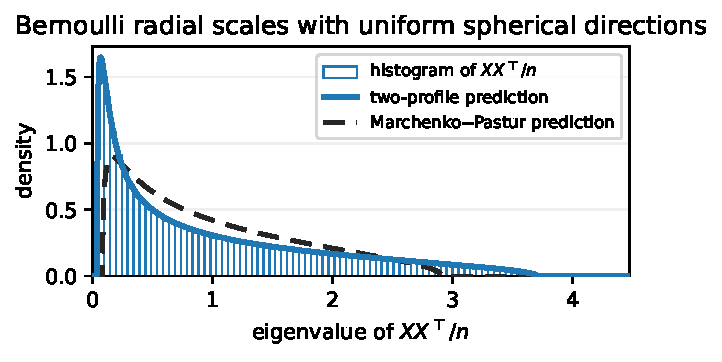
\includegraphics[width=\linewidth]
        {radial_mixture_with_two_profile_surrogate.pdf}
\end{minipage}
\end{landscape}
